\documentclass[11pt]{amsart}

\usepackage{lmodern}
\usepackage[T1]{fontenc}
\usepackage{amsmath,amssymb,amsthm}
\usepackage{booktabs}
\usepackage{tikz}
\usetikzlibrary{arrows.meta,positioning}
\usepackage{pgfplots}
\pgfplotsset{compat=1.17}
\usepackage[margin=1in]{geometry}
\usepackage{microtype}
\usepackage[hidelinks]{hyperref}

\theoremstyle{plain}
\newtheorem{theorem}{Theorem}[section]
\newtheorem{proposition}[theorem]{Proposition}
\theoremstyle{definition}
\newtheorem{definition}[theorem]{Definition}
\newtheorem{remark}[theorem]{Remark}

\newcommand{\code}[1]{\texttt{#1}}
\newcommand{\fpemu}{\code{fp64-emu}}
\newcommand{\gemmul}{\code{GEMMul8}}

\setlength{\emergencystretch}{3em}

\begin{document}

\title[Range-adaptive residue emulation of FP64 GEMM]{Range-Adaptive Double-Precision GEMM Emulation on Integer Tensor Cores with Exact Residue Reconstruction}
\author{Charles C. Norton}
\date{July 2026}
\subjclass[2020]{Primary 65Y04, 65F30; Secondary 65Y05, 68W10}
\keywords{matrix multiplication, DGEMM emulation, integer tensor cores, Chinese Remainder Theorem, Ozaki scheme, mixed-precision computing, GPU computing}

\begin{abstract}
Most consumer and workstation GPUs execute double-precision arithmetic at
one sixty-fourth of their single-precision rate, while their INT8 tensor
cores are the fastest units on the die. We present RARE, range-adaptive
residue emulation, implemented in the open library \fpemu{}:
double-precision matrix multiplication executed as one INT8 GEMM per
pairwise-coprime modulus and recovered exactly through the Chinese
Remainder Theorem, following the Ozaki-II scheme. A runtime
Cauchy--Schwarz pass measures the operands and converts unused residue
range into operand precision, making every modulus count range-safe;
extraction runs entirely in integer arithmetic with round-to-nearest
splitting, and two additional INT8 GEMMs cancel the first-order
quantization error; reconstruction computes balanced mixed-radix digits
with packed byte dot products held in registers; and a fused tensor-core
engine reduces every product to a one-byte residue in its epilogue,
dispatched against cuBLAS by measured per-shape timing. We prove range
safety, bit-exactness on representable inputs, and a worst-case error
bound that quantifies the correction. Measured on five NVIDIA
architectures, \fpemu{} exceeds native FP64 by up to a factor of 26 on
the FP64-throttled parts and exceeds \gemmul{}, the scheme authors'
reference implementation, at every size on every such part at equal GEMM
counts, by 1.07 to 3.80 times; on unthrottled datacenter silicon,
emulation pays only at scale, and there \gemmul{} leads. A tiled Cholesky
factorization routing its trailing updates through the batched entry
point runs 1.5 times faster end to end at equal residuals. Accuracy
exceeds native DGEMM in every distribution tested, with exactness
verified against integer oracles to depth $200{,}000$.
\end{abstract}

\maketitle

\section{Introduction}

The arithmetic that modern GPUs are best at is not the arithmetic that
scientific computing asks for. A current consumer or workstation GPU
executes IEEE double precision at $1/64$ of its single-precision rate: an
RTX 6000 Ada sustains roughly $1.3$ TFLOP/s in FP64 against hundreds of
tera-operations per second on its INT8 tensor cores, and the recent
Blackwell workstation parts widen this ratio further. Deep learning
workloads dominate the economics of GPU design, and full-rate
double-precision units survive only on a shrinking set of datacenter
parts. For the large community computing on everything else, double-precision matrix
multiplication is effectively a legacy path executed at a small fraction of
the machine's capability.

Emulation inverts this situation. If a double-precision product can be
decomposed into a modest number of low-precision matrix multiplications,
the idle tensor cores pay for the decomposition many times over. The
question is what the decomposition costs in accuracy, generality, and
overhead, and the answer has improved in three generations of work. The
Ozaki scheme \cite{ozaki2012} splits each operand into high-precision
slices and forms the product as a sum of error-free partial products;
mapped onto integer tensor cores by Ootomo, Ozaki, and Yokota
\cite{ootomo2024} and refined by Uchino, Ozaki, and Imamura
\cite{uchino2025}, it emulates DGEMM with a number of low-precision GEMMs
that grows quadratically in the slice count. The Ozaki-II scheme of Ozaki,
Uchino, and Imamura \cite{ozaki2scheme} replaces slicing with residue
arithmetic: the scaled integer operands are reduced modulo a set of small
pairwise-coprime moduli, one INT8 GEMM computes the product in each residue
class, and the Chinese Remainder Theorem recovers the exact integer
product. The modulus count, and with it the GEMM count, is now linear in
the recovered precision. The authors' open-source library, \gemmul{}
\cite{gemmul8repo}, is the reference implementation of this scheme and the
measured state of the art.

This paper presents RARE, a range-adaptive residue emulation of
double-precision GEMM implemented in the \fpemu{} library. On the
architectures whose FP64 units are throttled, which are the parts this
class of method exists for, it is faster than \gemmul{} at every size at
equal GEMM counts, while extending the scheme's guarantees in several
directions. The contributions are as follows.

\emph{Runtime operand sizing (Section~\ref{sec:sizing}).} Ozaki-II sizes
its integerization from a worst-case bound: the user fixes the modulus
count, and the scaling width $k$ is derived so that even $K$ fully aligned
terms at full magnitude cannot overflow the residue range. Real data sits
far below this worst case. \fpemu{} measures the operands at run time, in
one pass fused with the scaling pass, and applies the Cauchy--Schwarz
inequality to bound the actual product: whatever residue range the data
leaves unused is converted into additional operand mantissa bits, and when
the data needs more range than the configured moduli provide, the operands
are narrowed instead. The consequence is a scheme in which every modulus
count is unconditionally safe. Adversarial input costs correct bits; it
cannot corrupt the answer.

\emph{Integer-only extraction with first-order correction
(Section~\ref{sec:extract}).} The pass that converts scaled doubles into
balanced residues is memory-bound in principle but was compute-limited in
practice: on parts whose FP64 pipe runs at $1/64$ rate, even the handful of
floating-point operations in a rounding-and-scaling step co-limits the
kernel. Our extraction operates on the raw IEEE encoding in integer
registers throughout, performing round-to-nearest-even by explicit shift
arithmetic and reducing each scaled integer to all residues through a
three-limb 32-bit Barrett scheme. Where Ozaki-II truncates toward zero and
controls the resulting error through its worst-case width, we round to
nearest and then cancel the first-order quantization error explicitly: two
additional INT8 GEMMs over eight-bit summaries of the operands and their
residuals recover the cross terms, lifting accuracy past the ceiling that
operand quantization alone imposes and making the default configuration
more accurate than native DGEMM.

\emph{Register-resident balanced-Garner reconstruction
(Section~\ref{sec:recon}).} Ozaki-II reconstructs through the classical CRT
sum, accumulating $C_i \cdot M_i \cdot y_i$ in wide arithmetic and reducing
modulo the full modulus product. We instead compute balanced mixed-radix
digits by Garner's recurrence, reformulated so that the digit inner
products run as packed byte-dot-product (\code{dp4a}) instructions over
digits held four to a register, and the final recombination collapses to
one 64-bit Horner step per group of seven moduli. The kernel keeps every
intermediate in registers; on the architecture where this pass was
compute-bound, the reformulation made it $1.6\times$ faster, and the exact
path produces the correctly rounded double of the reconstructed integer.

\emph{A fused residue engine with measured dispatch
(Section~\ref{sec:engine}).} \gemmul{} executes its modular products
through cuBLAS INT8 GEMMs into full 32-bit product planes that a separate
pass reduces. \fpemu{} carries an in-file tensor-core kernel whose epilogue
Barrett-reduces every product to its balanced residue and stores one byte
per element, quartering the intermediate traffic; its operands are staged
through a tile-blocked layout written by the extraction pass in exactly the
order the kernel consumes, and on Hopper and Blackwell the staging uses the
Tensor Memory Accelerator. Because neither engine wins everywhere, the
dispatcher times both once per problem shape and caches the choice, a
policy that remains correct on architectures we never measured. The same
infrastructure supports batched products through plane-batch slots,
consumption of the standard $[K, N]$ operand layout without a transpose
copy, products of depth up to $K = 8.4$ million through segmented residue
accumulation, and capture into CUDA graphs, under which the emulation
outpaces native FP64 from matrix dimension 64 upward.

\emph{Measurement (Section~\ref{sec:eval}).} We evaluate on five NVIDIA
architectures: GeForce RTX 3070~Ti (consumer Ampere, SM~8.6), RTX 6000
Ada (SM~8.9), RTX PRO 6000 Blackwell Server Edition (SM~12.0),
A100-SXM4-80GB (datacenter Ampere, SM~8.0), and H200 (Hopper, SM~9.0).
Against native FP64, the default configuration reaches $26.1\times$ at
$n = 8192$ on Blackwell at accuracy above native DGEMM in every
distribution and depth combination tested. Against \gemmul{}, built from
source and measured on the same hardware with the GEMM count held equal,
\fpemu{} is faster at every size on the three throttled parts, by
$1.07\times$ to $3.80\times$; on Hopper, whose FP64 is unthrottled,
\gemmul{} leads at the largest sizes. On exactly representable inputs the
default reproduces the true product bit for bit, verified by equality
against integer oracles including an adversarial fully aligned case and a
dyadic dynamic-range case.

The implementation is a single CUDA source file with a Python surface,
published with all measurement scripts \cite{fpemurepo}.

\section{Background and Related Work}\label{sec:background}

\subsection{The Ozaki line}

The original Ozaki scheme \cite{ozaki2012} is an error-free transformation
of matrix multiplication: each operand is split into slices whose products
are exactly representable, so a high-precision product becomes a sum of
low-precision GEMMs. Its appeal on modern hardware is that the low-precision
GEMMs can be executed by matrix engines; Mukunoki, Ozaki, Ogita, and
Imamura demonstrated DGEMM on FP16 tensor cores this way
\cite{mukunoki2020}, and Ootomo, Ozaki, and Yokota moved the scheme to
integer units \cite{ootomo2024}, where the multiply-accumulate is exact and
the slice products are error-free by construction. Uchino, Ozaki, and
Imamura \cite{uchino2025} improved the integer variant's accuracy and
throughput. The cost structure of all slicing schemes is quadratic: $s$
slices per operand require $s(s+1)/2$ GEMMs.

Ozaki-II \cite{ozaki2scheme} abandons slicing for residue arithmetic.
Operands are scaled by powers of two and truncated to integers; each
integer matrix is reduced modulo $s$ pairwise-coprime moduli chosen so
that balanced residues fit INT8; one INT8 GEMM per modulus computes the
product in each residue class, exactly, because a sum of products of
values bounded by $128$ in magnitude stays within INT32 for any practical
inner dimension; and the true integer product is recovered from its
residues by the Chinese Remainder Theorem, provided it lies within the
signed range of the modulus product. The GEMM count is now linear in the
recovered precision: roughly eight bits per modulus. The reference
implementation \gemmul{} executes the modular GEMMs through
\code{cublasGemmEx} and exposes the modulus count and a fast/accurate mode
pair as tuning parameters; its fast mode estimates the output magnitude by
the Cauchy--Schwarz inequality, while its accurate mode spends one
additional INT8 GEMM to compute the bound exactly and reduce the scaling
overestimate. We adopt from \gemmul{} its modulus table, whose composite
entries ($255 = 3 \cdot 5 \cdot 17$, $253$, $247$, $217$) carry nearly
eight bits each where primes alone would carry fewer; balanced residues
make the ceiling $256$ rather than $128$, since the symmetric
representative range $[-(m-1)/2, m/2]$ of $m = 256$ lands exactly on the
INT8 domain.

\subsection{Other emulation paths}

NVIDIA has announced floating-point emulation inside cuBLAS itself
\cite{nvidiablog}, currently centered on FP32 emulation via BF16 tensor
cores, with FP64 support on datacenter parts; the numerical behavior of
tensor-core arithmetic that such schemes build on is analyzed in
\cite{fasi2021,markidis2018}. Mixed-precision iterative refinement
\cite{haidar2018} attacks the same economics from the solver side,
running factorizations in low precision and recovering accuracy through
residual iteration; emulated DGEMM is complementary, serving the many
workloads that want a drop-in high-precision product rather than a
restructured solver. Since the Ozaki-II preprint, an FP8 variant
\cite{fp8ozaki} and fused-kernel treatments \cite{emugemm} have appeared,
and the scheme has been evaluated inside factorization workloads
\cite{factorizations}; these confirm an active design space in which the
measured comparison of Section~\ref{sec:eval} situates our contribution.

\section{The Pipeline}\label{sec:method}

Figure~\ref{fig:pipeline} shows the five phases of RARE as implemented in
\fpemu{}. This section
walks through the numerically substantive ones: the sizing pass that
chooses the operand width, the extraction that produces residues and
correction operands, and the reconstruction. Section~\ref{sec:engine}
covers the engine that executes the modular GEMMs and the dispatch
machinery around it.

\begin{figure}[t]
\centering
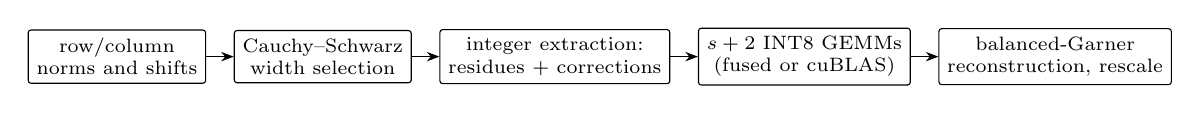
\begin{tikzpicture}[
  node distance=3mm and 3.5mm,
  box/.style={draw, rounded corners=1pt, align=center, inner sep=3pt, font=\scriptsize},
  arr/.style={-{Stealth[length=1.6mm]}}
]
\node[box] (scale) {row/column\\norms and shifts};
\node[box, right=of scale] (size) {Cauchy--Schwarz\\width selection};
\node[box, right=of size] (ext) {integer extraction:\\residues + corrections};
\node[box, right=of ext] (gemm) {$s+2$ INT8 GEMMs\\(fused or cuBLAS)};
\node[box, right=of gemm] (rec) {balanced-Garner\\reconstruction, rescale};
\draw[arr] (scale) -- (size);
\draw[arr] (size) -- (ext);
\draw[arr] (ext) -- (gemm);
\draw[arr] (gemm) -- (rec);
\end{tikzpicture}
\caption{The \fpemu{} pipeline. All five phases execute on the GPU; the
sizing decision is made on device, so no synchronization with the host
occurs between phases.}
\label{fig:pipeline}
\end{figure}

\subsection{Scaling and runtime operand sizing}\label{sec:sizing}

Both the slicing and residue schemes begin the same way: each row of $A$
and each column of $B$ is scaled by a power of two so that its largest
element becomes an integer carrying the leading mantissa bits. Writing
$\tilde{A} = \mathrm{round}(A \, 2^{\sigma_i})$ row-wise with
$|\tilde{A}_{ij}| < 2^{b}$, the exact integer product
$P = \tilde{A}\tilde{B}$ determines $C = AB$ up to the per-row and
per-column power-of-two rescale, and the whole numerical question becomes
whether $P$ fits inside the signed range $M/2$ of the modulus product
$M = \prod_i m_i$ and how much of each operand's mantissa the width $b$
retains.

The tension is that these two quantities trade against each other through
a bound that is almost never tight. In the worst case, an inner product of
$K$ terms, each the product of two $b$-bit integers of the same sign at
full magnitude, requires $2b + \lceil \log_2 K \rceil + 1$ bits. Ozaki-II
provisions for exactly this case: given the user's modulus count, it
derives the width from the worst-case rule, which for random data wastes
most of the provisioned range, since a random inner product grows like
$\sqrt{K}$ rather than $K$.

\fpemu{} measures instead. The scaling pass, which must in any case scan
every element once to find each row's maximum, additionally accumulates
each row's 2-norm. By the Cauchy--Schwarz inequality,
\[
  |P_{ij}| \;=\; \Bigl|\sum_k \tilde{A}_{ik}\tilde{B}_{kj}\Bigr|
  \;\le\; \|\tilde{A}_{i,:}\|_2 \, \|\tilde{B}_{:,j}\|_2
  \;\le\; \max_i \|\tilde{A}_{i,:}\|_2 \cdot \max_j \|\tilde{B}_{:,j}\|_2,
\]
a rigorous bound computable from two scalar reductions. A second, tiny
kernel compares this bound against the configured range $\log_2 M$ and
chooses the largest additional shift $g$ such that widening both operands
by $g$ bits, which scales the product bound by $2^{2g}$, still fits with
half a bit of margin; the margin dominates both the rounding slack of the
scaled integers and the accumulation error of the norm reduction. The
shift folds into the per-row scales, and the rest of the pipeline sees a
single effective width $b_{\mathrm{eff}} = b + g$.

Two consequences follow. First, on typical data the default configuration
recovers the full 53-bit significand with fewer moduli than the worst-case
rule would demand, because the measured bound sits near
$\log_2 K / 2 + 2b$ rather than $\log_2 K + 2b$. Second, and more
important for robustness, $g$ may be negative: if the caller provisions
fewer moduli than the data requires, the operands are narrowed until the
bound fits. Every modulus count is therefore unconditionally range-safe,
and the count becomes a pure accuracy-versus-speed knob. \gemmul{}'s fast
mode also invokes Cauchy--Schwarz, but for a different purpose, estimating
the output magnitude to set its scaling constant against a fixed width;
there, an overestimate costs accuracy. Here the inequality allocates the
width itself, and an overestimate merely leaves a fraction of a bit
unclaimed. We additionally cap the usable range at $2^{126}$ so that the
128-bit reconstruction path of Section~\ref{sec:recon} remains sound at
any depth; the cap is invisible below twenty moduli.

The bound degrades gracefully on adversarial input. For fully aligned
data, all terms of one sign at full magnitude, the norms detect exactly
the worst case and the operands narrow accordingly; the test suite
includes an all-ones product at $K = 2048$, reproduced exactly.
Non-finite data drives the norm to
infinity, which disables widening and falls back to the worst-case rule.

\subsection{Integer-only extraction and the correction planes}\label{sec:extract}

The extraction pass reads each scaled double once and writes $s$ residue
planes plus two correction operands. It is, by construction, a streaming
pass whose floor is memory bandwidth, and reaching that floor required
removing every FP64 instruction from it: on SM~8.6, profiling attributed a
co-limiting share of the pass to the $1/64$-rate FP64 pipe through the
\code{nearbyint}/\code{ldexp} formulation. The shipped kernel therefore
operates on the raw IEEE encoding in integer registers. The power-of-two
scale is an exponent addition; round-to-nearest-even of
$\mathrm{mag} \cdot 2^{-t}$ is an explicit shift with tie handling on the
retained low bit; and the result, biased by $2^{b_{\mathrm{eff}}}$ to make
it non-negative, splits into three 18-bit limbs from which each balanced
residue follows by
\[
  r \;=\; \bigl(\ell_2 c_{36} + \ell_1 c_{18} + \ell_0 + c_b\bigr) \bmod m,
  \qquad c_{36} = 2^{36} \bmod m,\; c_{18} = 2^{18} \bmod m,
\]
with $c_b$ chosen to cancel the bias inside the sum. The limb sum stays
below $2^{26}$, so a single 32-bit Barrett multiplication with one
conditional subtraction reduces it; no 64-bit multiply-high appears
anywhere in the pass. The integer formulation is also exact where an
underflowing \code{ldexp} would round. Measured in isolation, the pass
runs at 92\% of DRAM bandwidth on SM~8.6.

Rounding to nearest halves the worst-case quantization residual relative
to Ozaki-II's truncation, but the more consequential departure is that we
then cancel the first-order error explicitly. Write
$\tilde{A} + r_A = A \, 2^{\sigma}$ with $|r_A| \le \tfrac12$
element-wise. The exact product decomposes as
\[
  A 2^{\sigma} \, B 2^{\tau}
  \;=\; \tilde{A}\tilde{B}
  \;+\; \bigl(\tilde{A} r_B + r_A \tilde{B}\bigr)
  \;+\; r_A r_B ,
\]
and the middle term, the first-order quantization error, is itself a pair
of matrix products over small operands. During extraction we emit, per
element, an eight-bit summary $h = \mathrm{round}(\tilde{A} \,
2^{7-b_{\mathrm{eff}}})$ of the integer's leading bits and an eight-bit
quantization residual $q = \mathrm{round}(r \cdot 2^{8})$, both spanning
the full signed INT8 range. Two additional INT8 GEMMs, $h_A q_B^{\top}$
and $q_A h_B^{\top}$, then recover the first-order term at scale
$2^{b_{\mathrm{eff}} - 15}$, and the reconstruction folds it in before the
single final rounding. On integer inputs the residuals vanish identically
and the correction is exact silence. On general inputs the correction
lifts accuracy roughly four bits past the quantization ceiling, which is
what carries the default configuration above native DGEMM
(Section~\ref{sec:accuracy}); it costs two GEMMs against the roughly
fourteen the default already runs. Ozaki-II has no analogous term; its
accurate mode spends its extra GEMM on a tighter magnitude bound rather
than on error cancellation.

\subsection{Reconstruction}\label{sec:recon}

After the modular GEMMs, each output element exists as $s$ balanced
residues, and the remaining work is to recover the integer they encode and
scale it into the output double. This pass is elementwise: at
$s \approx 14$ moduli it reads fourteen bytes of residues and eight of
correction data per element while performing an $O(s^2)$ digit recurrence,
a profile that is neither bandwidth-bound nor negligible.

We reconstruct by Garner's mixed-radix recurrence rather than by the
classical CRT sum that Ozaki-II uses. The mixed-radix digits
\[
  d_t \;=\; \Bigl( r_t - \sum_{u < t} d_u \,(M_u \bmod m_t) \Bigr)
  \, (M_t \bmod m_t)^{-1} \bmod m_t,
  \qquad M_u = \prod_{v<u} m_v,
\]
computed in the balanced representative range, are bounded by $m_t/2$ and
therefore fit signed bytes, and every factor $M_u \bmod m_t$ can be
re-balanced to a byte as well without leaving its congruence class. The
inner product of the recurrence then becomes a dot product of two
byte-vectors, which GPUs execute four lanes at a time by the \code{dp4a}
instruction. We pack the digits four to a 32-bit register as they are
produced and pre-pack the factor table with zeros above the diagonal, so
each digit costs a fixed number of \code{dp4a} operations, one 32-bit
Barrett reduction, and no tail handling: at nineteen prior digits the
whole recurrence step stays below $2^{19}$ and never needs 64-bit
arithmetic.

The final recombination $P = \sum_t d_t M_t$ is a Horner evaluation whose
naive form costs one 128-bit multiply-add per modulus, and profiling on
SM~8.6 showed the kernel bound on the pipe that executes wide integer
multiplies. We collapse the evaluation into groups: a Horner pass over at
most seven moduli stays below $2^{55}$ and runs in plain 64-bit registers,
and the groups combine high to low with a single wide multiply each,
$P = a_0 + M_{0..6}\,(a_1 + M_{7..13}\, a_2)$. Two wide multiplies replace
thirteen 128-bit steps at the default modulus count. A register-residency
constraint completes the design: both digit loops unroll to the
compile-time modulus maximum and exit at the runtime count, because any
runtime-indexed thread-local array is demoted to local memory, which we
measured as a $2.4\times$ amplification of the kernel's DRAM traffic. The
grouped, register-resident form made the reconstruction $1.6\times$ faster
on SM~8.6 and $1.4\times$ faster on SM~8.9, and left it at its measured
traffic floor on the latter.

The exact path performs the recombination in 128-bit integer arithmetic
carried as two 64-bit halves, adds the correction term at its scale, and
converts once to double with correct rounding, folding the dropped tail
into a sticky bit far below the round position. The result is the
correctly rounded double of the corrected integer product. A fast path
replaces the 128-bit combine with one in double precision, trading the
last bit of the accumulator for a few percent of the phase; both paths
keep the recombination off the throttled native-FP64 pipe.

\subsection{Guarantees}\label{sec:guarantees}

The pipeline's numerical claims reduce to three statements: the sizing
pass never admits a product that wraps the residue range, the arithmetic
between extraction and output is exact, and the correction bounds the
error on general inputs. We state and prove them here; throughout,
$b_e$ denotes the effective operand width, $\sigma_i$ and $\tau_j$ the
per-row and per-column shifts after widening,
$\tilde{a}_{ik} = \mathrm{round}(a_{ik} 2^{\sigma_i})$ with residual
$r^A_{ik} = a_{ik} 2^{\sigma_i} - \tilde{a}_{ik}$, $|r^A_{ik}| \le
\tfrac12$, and $P = \tilde{A} \tilde{B}^{\top}$ the exact integer
product. $M^{*} = \min(\prod_t m_t,\, 2^{126})$ is the capped range.

\begin{proposition}[Range safety]\label{prop:range}
Let $b_e \ge 16$ and $K \le 2^{23}$, and suppose the widening pass
accepts the shift under its half-bit margin, that is,
$\lambda_A + \lambda_B + \tfrac12 \le \log_2 M^{*} - 1$, where
$\lambda_A$ is the computed value of
$\max_i \log_2 \| a_{i,:} 2^{\sigma_i} \|_2$ and likewise $\lambda_B$.
Then $|P_{ij}| < M^{*}/2$ for all $i, j$: the balanced CRT representative
of every output element is $P_{ij}$ itself, and the 128-bit recombination
cannot overflow.
\end{proposition}

\begin{proof}
By Cauchy--Schwarz, $|P_{ij}| \le \|\tilde{a}_{i,:}\|_2
\|\tilde{b}_{:,j}\|_2$. Rounding perturbs each row norm by at most
$\tfrac{\sqrt{K}}{2}$ in absolute terms, and the scaled row maximum is at
least $2^{b_e - 1}$, so
$\|\tilde{a}_{i,:}\|_2 \le \|a_{i,:} 2^{\sigma_i}\|_2 (1 + \sqrt{K}\,
2^{-b_e})$, an inflation of at most $\log_2(1 + 2^{11.5 - 16}) < 0.064$
bits under the stated hypotheses, and likewise for columns. The norm
itself is accumulated in binary64, whose relative error over at most $K$
terms is below $2^{-30}$, and stored in binary32, contributing less than
$2^{-15}$ bits; the shifts are powers of two and perturb nothing. The
total slack on the left-hand side is therefore below
$2 \cdot 0.064 + 2^{-14} < \tfrac12$, so the true bound satisfies
$\log_2 (\|\tilde{a}_{i,:}\| \|\tilde{b}_{:,j}\|) \le \lambda_A +
\lambda_B + \tfrac12 \le \log_2 M^{*} - 1$.
\end{proof}

\begin{proposition}[Exactness]\label{prop:exact}
Under Proposition~\ref{prop:range}, the exact path returns
$\mathrm{RN}\bigl(2^{-\sigma_i - \tau_j} (P_{ij} + 2^{b_e - 15}
\Delta_{ij})\bigr)$, the correctly rounded double of the corrected
integer value, where $\Delta$ is the integer carried by the two
correction GEMMs. In particular, when every scaled entry is an integer,
the residuals vanish, $\Delta = 0$, and the output is the correctly
rounded true product; when that product is representable, the result is
exact.
\end{proposition}

\begin{proof}
Each stage is exact integer arithmetic. The three-limb residues are
computed from the biased integer without rounding; each modular GEMM
accumulates products of balanced residues bounded by $128$ in magnitude,
so a single launch stays within int32 for $K < 2^{17}$ and the segmented
path within its int32 residue accumulators, whose entries are bounded by
$128$ per segment over at most $128$ segments. The balanced mixed-radix
digits are the unique such representation of $P_{ij} \bmod \prod m_t$,
and by Proposition~\ref{prop:range} that representative is $P_{ij}$. The
grouped recombination and the correction addition are exact in 128-bit
integer arithmetic within the $2^{126}$ cap, and the conversion folds the
dropped tail into a sticky bit strictly below the round position, which
preserves round-to-nearest-even. When the residuals vanish, both
correction operands $q$ are identically zero, so $\Delta = 0$
identically. The test suite witnesses the claim by bit equality against
integer oracles, including the aligned worst case, a dyadic
dynamic-range case, and, through the segmented path, $K = 200{,}000$.
\end{proof}

\begin{proposition}[Accuracy after correction]\label{prop:accuracy}
Let $S_{ij} = \sum_k (a_{ik} 2^{\sigma_i}) (b_{kj} 2^{\tau_j})$ be the
exact scaled product and $V_{ij} = P_{ij} + 2^{b_e-15} \Delta_{ij}$ the
corrected value. With the eight-bit summaries clamped to $[-127, 127]$,
\[
  |V_{ij} - S_{ij}|
  \;\le\; K \Bigl( 3 \cdot 2^{b_e - 8} + 2^{b_e - 15} + \tfrac14 \Bigr),
\]
and the returned double adds one rounding at the output scale. Without
the correction GEMMs the corresponding bound is $K \cdot 2^{b_e}$, so
the correction is worth seven bits in the worst case.
\end{proposition}

\begin{proof}
Write $S - P = \sum_k (\tilde{a} r^B + r^A \tilde{b} + r^A r^B)$
element-wise. The summaries satisfy $h = \tilde{a} 2^{7 - b_e} + e_h$ and
$q = r 2^{8} + e_q$, where rounding alone gives $|e| \le \tfrac12$ and
the clamp at $\pm 127$ raises the bound to $|e| \le \tfrac32$ (the
unclamped values reach $\pm 128$). Expanding one correction pair,
\[
  2^{b_e - 15} h_a q_b
  \;=\; \tilde{a}\, r^B
  \;+\; \tilde{a}\, 2^{-8} e_q
  \;+\; e_h\, r^B\, 2^{b_e - 7}
  \;+\; e_h e_q\, 2^{b_e - 15},
\]
whose error terms are bounded by $\tfrac32 \cdot 2^{b_e - 8}$,
$\tfrac34 \cdot 2^{b_e - 7}$, and $\tfrac94 \cdot 2^{b_e - 15}$
respectively; the symmetric pair contributes the same, and the
uncorrected second-order term is $|r^A r^B| \le \tfrac14$. Summing over
$K$ terms and collecting constants gives the stated bound. Without the
correction the first-order term alone contributes up to
$2 \cdot 2^{b_e - 1} = 2^{b_e}$ per term.
\end{proof}

The bound explains the measured behavior: at $b_e$ near $53$ the
corrected worst case sits roughly seven bits below the uncorrected
ceiling, and the four to five bits observed on random data
(Section~\ref{sec:accuracy}) are the root-mean-square realization of it.
The clamp affects only entries whose residual magnitude exceeds
$\tfrac{255}{512}$ and costs at most a factor of three in the dominant
constant.

\section{The Engine and Its Dispatch}\label{sec:engine}

\subsection{A fused residue GEMM}

The modular products themselves are ordinary INT8 GEMMs, and \gemmul{}
delegates them to cuBLAS. Doing so fixes two costs.
First, cuBLAS writes 32-bit accumulators, so $s + 2$ full INT32 product
planes must be materialized and then reduced by a separate pass, a
round-trip of $4(s+2)$ bytes per output element. Second, a library GEMM
consumes row-major operands at a fixed layout, which constrains the
extraction pass to a write pattern that the GEMM then re-reads
inefficiently.

\fpemu{} carries its own tensor-core kernel for these products. The kernel
computes $128 \times 256$ output tiles per thread block on
\code{mma.sync.m16n8k32} fragments, eight warps each owning a
$64 \times 64$ warp tile so that thirty-two tensor-core operations issue
behind every eight fragment loads; operands stream through a four-slot
shared-memory ring synchronized by per-slot arrival barriers with no
block-wide synchronization in the main loop. Its distinguishing feature is
the epilogue: each 32-bit accumulator is Barrett-reduced to its balanced
residue inside the epilogue and stored as one byte, directly from
registers, eliminating the INT32 planes and the reduction pass entirely.
The correction products, which must remain 32-bit, share the same launch
as two additional plane slots. On SM~9.0 and SM~12.0 the operand staging
uses the Tensor Memory Accelerator with hardware swizzling; below that,
asynchronous copies stage a tile-blocked operand layout that the
extraction pass writes in exactly the order the kernel consumes, turning
the staging into contiguous streaming reads. Ragged edges are zero-padded
at extraction, so the kernel carries no bounds checks in its hot loop, and
none of $M$, $N$, $K$ carries an alignment constraint, unlike the
INT8 paths of cuBLAS or \code{torch.\_int\_mm}.

\subsection{Measured dispatch}

Neither engine dominates. The fused kernel wins wherever its byte-wide
epilogue traffic and fused reduction outweigh cuBLAS's higher raw GEMM
throughput, which happens at small and medium sizes on every architecture
and at all sizes on some; cuBLAS wins at the largest sizes on the parts
where its INT8 kernels are strongest. The crossover moves with
architecture, size, and modulus count, and any fixed rule encodes a guess
that the next GPU falsifies. \fpemu{} instead times the viable candidates
once per problem shape, on the first call, warmed to exclude one-time
setup, and caches the winner; the same policy chooses between cuBLAS's
strided-batched call and a per-plane loop, whose relative speed also
inverts across architectures. When the INT32 planes of the cuBLAS path
would not fit free memory, a chunked variant multiplies groups of planes
into a bounded buffer and reduces each group to residues before the next
runs. Environment overrides pin any path for measurement, and every path
computes bit-identical results, which the test suite asserts.

\subsection{Extensions}\label{sec:extensions}

Three extensions widen the applicable surface without altering the
numerics. \emph{Batching:} a uniform batch flattens into plane-batch
slots, so the whole batch shares one launch chain, one sizing pass with a
common operand width, and one reconstruction; per-call cost is paid once,
which at 64 products of dimension 256 makes the batched call
$4.5\times$ faster than looping on Blackwell and turns a regime where
emulation loses to native FP64 into one where it wins
(Section~\ref{sec:batched}). \emph{Layout:} the standard $[K, N]$ operand
is consumed in place, with per-column shifts gathered by coalesced
slab-reduction kernels and the residue planes written in the transposed
layout that cuBLAS's NN form consumes; the dispatcher weighs this
transpose-free path against the fused engine with an internal copy, and
the former removes a copy overhead of up to 14\% of runtime at mid sizes.
\emph{Depth:} products beyond the single-launch bound $K < 131072$, set
by the INT32 accumulator against balanced residues of magnitude 128, run
in segments of $65536$ whose balanced residues accumulate in INT32 planes,
bounded by $128$ per segment, and whose correction products accumulate in
INT64; one fold and one reconstruction close the sum, preserving
bit-exactness, which we verify at $K = 200{,}000$ against a CPU integer
oracle. All entry points register fake kernels for \code{torch.compile}
and are capturable into CUDA graphs; under graph replay, which removes the
host-side launch overhead that dominates small problems, the emulated
product outpaces native FP64 from $n = 64$ upward on SM~8.9.

\section{Evaluation}\label{sec:eval}

\subsection{Setup}

We measure on five NVIDIA architectures: GeForce RTX 3070 Ti Laptop
(consumer Ampere, SM~8.6, 8 GB), RTX 6000 Ada (SM~8.9, 48 GB), RTX PRO
6000 Blackwell Server Edition (SM~12.0), A100-SXM4-80GB (datacenter
Ampere, SM~8.0), and H200 (Hopper, SM~9.0). The first three throttle FP64
to $1/64$ of the FP32 rate; the last two do not, and the results divide
along exactly that line. Throughput is reported as $2n^3$ over the median
of 3 to 30 timed executions after warm-up, with iteration counts scaling
inversely with size; on the two locally held parts, which are thermally
variable, contending systems are additionally interleaved across repeated
rounds and each cell reports its best median. The Blackwell, A100, and
H200 numbers come from cloud instances. Native FP64 is
\code{torch.matmul} on the same tensors. Software per part: consumer
Ampere runs driver 580.126.09 with torch 2.7.1 on CUDA 12.6; Ada runs
torch 2.10.0 on CUDA 12.6 under Windows; the Blackwell, A100, and H200
instances run torch 2.8.0 on CUDA 12.9, 2.10.0 on CUDA 12.8, and 2.8.0
on CUDA 12.9 respectively. \gemmul{} is built at its revision
\code{6bf409b}. The first call at a new problem
shape additionally runs the dispatch probe and costs six to twelve times
the steady-state call (16.6 ms against 1.41 ms at $n = 2048$ on Ada), and
all timings exclude it. Accuracy is reported as correct bits, $-\log_2$
of the max-norm relative error against a reference accumulated in
double-double arithmetic and cross-checked against exact rational
arithmetic. The accuracy tables use $M = N = 128$: the error of both
systems is driven by the inner dimension $K$, not by the output extent,
and a spot check at $512 \times 4096 \times 512$ reproduces the pattern
(native 49.4 bits, default 53.2, reduced 44.6).

\gemmul{} is built from source and measured on the same hardware in every
comparison: through its direct interface compiled natively on Windows for
SM~8.9 and on Linux for SM~8.6, through its cuBLAS interposition hook on
SM~8.6 and SM~9.0, and compiled in situ on the cloud instances. Where two
measurement modes cover the same part they agree within three percent,
and its accuracy under our double-double reference matches its published
characterization, which cross-validates the harness.

The \fpemu{} \emph{default} configuration is self-sizing: fourteen moduli
plus the two correction GEMMs through $K = 8192$, fifteen plus two beyond.
The \emph{reduced} configuration drops one modulus and the correction
GEMMs, trading roughly eight bits of accuracy for speed. All numbers in
this section are reproduced by scripts in the artifact \cite{fpemurepo}.

\subsection{Throughput against native FP64}

Table~\ref{tab:native} summarizes the five architectures at $n = 8192$,
and Table~\ref{tab:blackwell} sweeps sizes on the part with the widest
FP64-to-INT8 ratio. The ratio to native tracks each part's throttling:
$26\times$ on Blackwell and $16\times$ on consumer Ampere, whose native
FP64 runs at $1/64$ rate, against $1.13\times$ on A100 and $1.02\times$
on H200, whose FP64 units are unthrottled and where emulation pays only
at scale. Below $n \approx 128$ per-call cost exceeds native on every
part; CUDA-graph replay moves this crossover to $n = 64$ on SM~8.9.
Figure~\ref{fig:sweep} plots the sweep on the three throttled parts.

\begin{figure}[t]
\centering
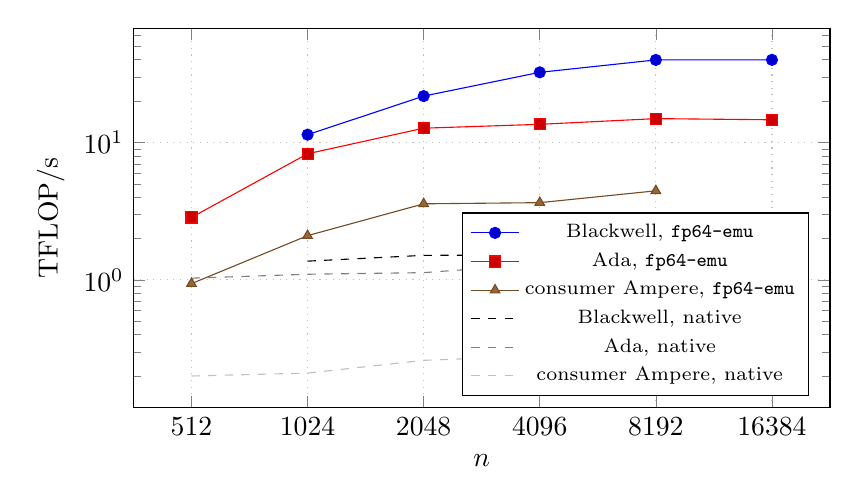
\begin{tikzpicture}
\begin{loglogaxis}[
  width=0.86\textwidth, height=6.4cm,
  xlabel={$n$}, ylabel={TFLOP/s},
  log basis x=2,
  xtick={512,1024,2048,4096,8192,16384},
  xticklabels={512,1024,2048,4096,8192,16384},
  legend pos=south east,
  legend style={font=\scriptsize},
  grid=major, grid style={dotted}
]
\addplot+[mark=*] coordinates
  {(1024,11.40) (2048,21.76) (4096,32.40) (8192,39.89) (16384,39.95)};
\addlegendentry{Blackwell, \fpemu{}}
\addplot+[mark=square*] coordinates
  {(512,2.85) (1024,8.28) (2048,12.71) (4096,13.56) (8192,14.92) (16384,14.63)};
\addlegendentry{Ada, \fpemu{}}
\addplot+[mark=triangle*] coordinates
  {(512,0.94) (1024,2.10) (2048,3.58) (4096,3.65) (8192,4.45)};
\addlegendentry{consumer Ampere, \fpemu{}}
\addplot+[dashed, mark=none, black] coordinates
  {(1024,1.37) (2048,1.51) (4096,1.52) (8192,1.53) (16384,1.53)};
\addlegendentry{Blackwell, native}
\addplot+[dashed, mark=none, gray] coordinates
  {(512,1.03) (1024,1.10) (2048,1.13) (4096,1.30) (8192,1.31) (16384,1.33)};
\addlegendentry{Ada, native}
\addplot+[dashed, mark=none, lightgray] coordinates
  {(512,0.20) (1024,0.21) (2048,0.26) (4096,0.28) (8192,0.28)};
\addlegendentry{consumer Ampere, native}
\end{loglogaxis}
\end{tikzpicture}
\caption{Default-configuration throughput against native FP64 on the
three FP64-throttled parts. Solid: \fpemu{}; dashed: native
\code{torch.matmul}.}
\label{fig:sweep}
\end{figure}

\begin{table}[t]
\centering
\caption{Throughput at $n = 8192$, square random-normal operands.
\emph{default} is the self-sizing configuration; \emph{reduced} drops one
modulus and the correction GEMMs.}
\label{tab:native}
\begin{tabular}{lcrrrrr}
\toprule
part & SM & native & default & vs.\ native & reduced & vs.\ native \\
\midrule
RTX PRO 6000 Blackwell & 12.0 & 1.53 TF & 39.89 TF & $26.1\times$ & 47.91 TF & $31.3\times$ \\
RTX 3070 Ti Laptop & 8.6 & 0.28 TF & 4.45 TF & $15.8\times$ & 5.25 TF & $18.7\times$ \\
RTX 6000 Ada & 8.9 & 1.31 TF & 14.92 TF & $11.4\times$ & 18.66 TF & $14.2\times$ \\
A100-SXM4-80GB & 8.0 & 17.58 TF & 19.91 TF & $1.13\times$ & 24.13 TF & $1.37\times$ \\
H200 & 9.0 & 58.18 TF & 59.50 TF & $1.02\times$ & 69.53 TF & $1.20\times$ \\
\bottomrule
\end{tabular}
\end{table}

\begin{table}[t]
\centering
\caption{RTX PRO 6000 Blackwell (Server Edition), SM 12.0, across sizes.}
\label{tab:blackwell}
\begin{tabular}{rrrrrr}
\toprule
$n$ & native & default & vs.\ native & reduced & vs.\ native \\
\midrule
256 & 0.41 TF & 0.60 TF & $1.5\times$ & 0.62 TF & $1.5\times$ \\
1024 & 1.37 TF & 11.40 TF & $8.3\times$ & 12.44 TF & $9.1\times$ \\
2048 & 1.51 TF & 21.76 TF & $14.4\times$ & 25.69 TF & $17.0\times$ \\
4096 & 1.52 TF & 32.40 TF & $21.3\times$ & 38.55 TF & $25.4\times$ \\
8192 & 1.53 TF & 39.89 TF & $26.1\times$ & 47.91 TF & $31.3\times$ \\
16384 & 1.53 TF & 39.95 TF & $26.0\times$ & 48.01 TF & $31.3\times$ \\
\bottomrule
\end{tabular}
\end{table}

\subsection{Comparison with GEMMul8}\label{sec:h2h}

The comparison of central interest is against the scheme's reference
implementation, and its fairness rests on configuring both systems at
their smallest FP64-equivalent settings. For \fpemu{} that is the
self-sizing default. For \gemmul{} we establish it by measurement:
Table~\ref{tab:g8sweep} sweeps its modulus count under our double-double
reference, and sixteen moduli reach the FP64-equivalent class at
$K = 4096$. Across depths, sixteen moduli hold $52.2$ to $53.3$ bits
through $K = 8192$ and measure $51.8$ on the spike distribution at
$K = 16384$, where seventeen restore $53.2$. Every comparison therefore
holds the GEMM count equal: \fpemu{}'s fourteen moduli plus two correction
GEMMs run against \gemmul{} at sixteen moduli, and fifteen plus two
against seventeen at $n = 16384$. \fpemu{} measures $53.1$ to $53.9$
correct bits across the grid and \gemmul{} measures $51.8$ to $53.3$, so
the equal-count pairing gives \gemmul{} the benefit of a slightly lower
accuracy floor.

\begin{table}[t]
\centering
\caption{\gemmul{} correct bits by modulus count, $K = 4096$,
random-normal / spike.}
\label{tab:g8sweep}
\begin{tabular}{lccccc}
\toprule
moduli & 14 & 15 & 16 & 17 & 18 \\
\midrule
bits & 48.1 / 46.3 & 52.3 / 50.2 & 53.0 / 52.7 & 53.0 / 53.3 & 53.0 / 53.2 \\
\bottomrule
\end{tabular}
\end{table}

\begin{table}[t]
\centering
\caption{Equal-GEMM-count throughput in TFLOP/s on the three
FP64-throttled architectures. Ratios are \fpemu{} over \gemmul{}. Dashes:
$n = 16384$ exceeds the 8 GB consumer part; the two smallest Blackwell
cells were not captured on the metered instance.}
\label{tab:gemmul8}
\small
\setlength{\tabcolsep}{4.5pt}
\begin{tabular}{r rrr rrr rrr}
\toprule
 & \multicolumn{3}{c}{consumer Ampere (8.6)} & \multicolumn{3}{c}{Ada (8.9)} & \multicolumn{3}{c}{Blackwell (12.0)} \\
\cmidrule(lr){2-4}\cmidrule(lr){5-7}\cmidrule(lr){8-10}
$n$ & ours & \gemmul{} & ratio & ours & \gemmul{} & ratio & ours & \gemmul{} & ratio \\
\midrule
512 & 0.94 & 0.64 & $1.47$ & 2.85 & 0.75 & $3.80$ & -- & -- & -- \\
1024 & 2.10 & 1.43 & $1.47$ & 8.28 & 4.40 & $1.88$ & -- & -- & -- \\
2048 & 3.58 & 2.27 & $1.58$ & 12.71 & 9.46 & $1.34$ & 21.76 & 13.14 & $1.66$ \\
4096 & 3.65 & 3.14 & $1.16$ & 13.56 & 12.20 & $1.11$ & 32.40 & 20.65 & $1.57$ \\
8192 & 4.45 & 3.80 & $1.17$ & 14.92 & 13.78 & $1.08$ & 39.89 & 30.78 & $1.30$ \\
16384 & -- & -- & -- & 14.63 & 13.72 & $1.07$ & 39.95 & 34.88 & $1.15$ \\
\bottomrule
\end{tabular}
\end{table}

Table~\ref{tab:gemmul8} reports the three throttled architectures, where
\fpemu{} is faster in every cell. The margin is largest at small sizes,
$3.80\times$ at $n = 512$ on Ada, where the fused single-launch pipeline
amortizes what \gemmul{}'s multi-kernel structure pays per call;
\gemmul{}'s small-$n$ throughput agrees across its Windows driver, Linux
driver, and Linux hook measurements on SM~8.6, so this cost is a property
of its pipeline rather than of any one platform. The margin narrows to
$7$ to $30$ percent at the largest sizes, where both systems converge
toward the throughput of the underlying INT8 GEMMs and the remaining
separation comes from the byte-wide epilogue, the extraction, and the
reconstruction.

Table~\ref{tab:hopper} reports Hopper, where the picture inverts at
scale: \fpemu{} leads at $n = 2048$, the systems are within a few percent
through $n = 8192$, and \gemmul{} leads by $13$ percent at $n = 16384$.
Hopper pairs unthrottled FP64 with exceptionally strong cuBLAS INT8
kernels, and \gemmul{}'s pipeline extracts more of that throughput at
scale than ours does; both systems trail native FP64 below $n = 8192$ on
this part.

\begin{table}[t]
\centering
\caption{Equal-GEMM-count throughput in TFLOP/s on H200 (Hopper, SM 9.0).}
\label{tab:hopper}
\begin{tabular}{rrrr}
\toprule
$n$ & \fpemu{} & \gemmul{} & ratio \\
\midrule
2048 & 22.63 & 19.95 & $1.13$ \\
4096 & 43.68 & 44.86 & $0.97$ \\
8192 & 59.50 & 58.61 & $1.02$ \\
16384 & 57.67 & 66.53 & $0.87$ \\
\bottomrule
\end{tabular}
\end{table}

At reduced precision, \fpemu{} at thirteen GEMMs against \gemmul{}'s
thirteen-modulus fast mode, the throttled-part pattern repeats at smaller
margins: $1.03\times$ to $2.92\times$ on consumer Ampere and Ada, and
$1.01\times$ to $1.38\times$ on Blackwell, against $0.74\times$ to
$0.97\times$ on Hopper. The one exception on the throttled parts is
$n = 16384$ on Ada, where the self-sizing range rule fields fourteen
moduli against thirteen and \gemmul{} leads by $6$ percent in proportion
to the extra GEMM; pinning thirteen moduli at that depth restores parity,
$17.28$ against $17.60$ TF, which localizes the deficit to the modulus
count rather than to any per-GEMM inefficiency.

\subsection{Component ablations}\label{sec:ablation}

Three of the contributions can be isolated. \emph{Sizing:} worst-case
provisioning for a 53-bit guarantee at $K = 4096$ requires sixteen moduli
(Section~\ref{sec:sizing}), eighteen GEMMs with the correction pair; the
runtime pass delivers 53.1 to 54.1 bits from fourteen moduli, sixteen
GEMMs, on all six distributions of Table~\ref{tab:accuracy}, a saving of
two GEMMs, narrowing to one at $K = 16384$. \emph{Engine:} pinning the
dispatch to one engine with everything else fixed separates the fused
kernel from cuBLAS. On Ada in a single interleaved sweep, the fused
engine delivers 7.34 against 5.30 TFLOP/s at $n = 1024$ and 12.52 against
11.39 at $n = 2048$, while the two agree within one percent at
$n = 8192$ (15.77 against 15.61); on consumer Ampere the ordering
inverts at large sizes, where the cuBLAS form leads by ten percent. No
fixed rule captures both parts, which is what the measured dispatch
replaces. \emph{Reconstruction:} the register-resident grouped form of
Section~\ref{sec:recon} is a component-level $1.6\times$ on SM~8.6 and
$1.4\times$ on SM~8.9 over the per-modulus 128-bit recurrence it
replaced.

\subsection{Accuracy}\label{sec:accuracy}

Table~\ref{tab:accuracy} reports correct bits on six input distributions
at two depths, measured on the Blackwell part; the reconstruction is
exact integer arithmetic and carries no architecture dependence, and spot
checks on the other parts agree within measurement spread. The
distributions include per-element exponent jitter of eight and sixteen
binades, shared column scalings spanning twenty and forty binades, and a
$2^{30}$ spike element per row.

\begin{table}[t]
\centering
\caption{Correct bits against a double-double reference, $M = N = 128$.
Native, default, and reduced are measured on the Blackwell part;
\gemmul{} at sixteen moduli is measured through its hook on consumer
Ampere, the reconstruction being architecture-independent. The default
exceeds native FP64 DGEMM in every cell.}
\label{tab:accuracy}
\begin{tabular}{lrrrrr}
\toprule
distribution & $K$ & native & default & reduced & \gemmul{} \\
\midrule
randn & 512 & 49.4 & 53.4 & 45.9 & 52.7 \\
randn & 4096 & 47.6 & 53.6 & 44.3 & 53.0 \\
wide8 & 512 & 49.4 & 53.7 & 46.2 & 52.9 \\
wide8 & 4096 & 47.6 & 53.7 & 45.1 & 52.5 \\
wide16 & 512 & 49.4 & 53.3 & 46.8 & 53.2 \\
wide16 & 4096 & 48.1 & 53.7 & 45.2 & 52.8 \\
illcond & 512 & 49.1 & 53.7 & 47.1 & 53.2 \\
illcond & 4096 & 47.7 & 53.3 & 45.4 & 52.6 \\
illcond40 & 512 & 49.6 & 53.6 & 48.6 & 52.9 \\
illcond40 & 4096 & 48.0 & 53.5 & 46.9 & 52.9 \\
spike & 512 & 48.7 & 54.0 & 45.7 & 53.3 \\
spike & 4096 & 47.8 & 53.2 & 43.3 & 52.7 \\
\bottomrule
\end{tabular}
\end{table}

The mechanism behind the uniform advantage over native DGEMM is
structural, not statistical: each emulated inner product is formed exactly
in the residue domain and rounded once, where native DGEMM accumulates
$K$ roundings, so the default sits at the output-rounding floor while
native drifts downward with depth. The exactness class is sharper still:
on representable inputs the product is bit-identical to exact arithmetic,
verified by equality against integer oracles across every dispatch path
and, through the segmented pipeline, at $K = 200{,}000$.

\subsection{Batched products}\label{sec:batched}

Iterative solvers and blocked factorizations, the workloads with the most
to gain from a fast accurate product, issue many small GEMMs rather than
one large one, and per-call overhead then dominates exactly where
emulation's raw advantage is thinnest. Table~\ref{tab:batched} measures
the batched entry point against native \code{torch.bmm} and against
looping the single-product call.

\begin{table}[t]
\centering
\caption{Batched throughput, RTX PRO 6000 Blackwell. The final column is
the speedup of the batched call over looping the single call.}
\label{tab:batched}
\begin{tabular}{lrrrr}
\toprule
batch $\times$ $n$ & native \code{bmm} & \fpemu{} \code{bmm} & vs.\ native & vs.\ loop \\
\midrule
$64 \times 256$ & 1.55 TF & 2.91 TF & $1.9\times$ & $4.5\times$ \\
$32 \times 512$ & 1.57 TF & 7.00 TF & $4.4\times$ & $1.6\times$ \\
$16 \times 1024$ & 1.58 TF & 13.92 TF & $8.8\times$ & $1.1\times$ \\
$8 \times 2048$ & 1.58 TF & 23.12 TF & $14.6\times$ & $1.1\times$ \\
$4 \times 4096$ & 1.59 TF & 32.71 TF & $20.5\times$ & $1.1\times$ \\
\bottomrule
\end{tabular}
\end{table}

The pattern on SM~8.9 is the same, $1.6\times$ to $9.7\times$ native
across the grid, and the loop amortization is architecture-independent:
on A100 and H200, where native FP64 keeps the absolute lead at these
sizes, batching remains $3.1\times$ and $4.0\times$ faster than looping
at $64 \times 256$. A batch of $64$ products of dimension $256$, a regime
where the single-call emulation only breaks even against native FP64 on
the throttled parts, runs at nearly twice native throughput batched.

\subsection{End to end: a tiled Cholesky factorization}\label{sec:e2e}

The batched entry point exists for blocked factorizations, so we close
the evaluation with one. A tiled right-looking Cholesky factorization
routes its trailing updates, batched tile products of uniform
$512^3$ GEMMs, through either \code{torch.bmm} or \code{emu.bmm}; the
panel factorization and triangular solves stay native in both
configurations, and both share identical gather and scatter code. On Ada
at $n = 16384$ the update phase drops from $1.23$ to $0.69$ seconds and
the whole factorization from $1.43$ to $0.94$ seconds, a $1.5\times$
end-to-end speedup; consumer Ampere at $n = 8192$ moves from $0.83$ to
$0.56$ seconds. The factorization residuals
$\|A - LL^{\top}\|_F / \|A\|_F$ are equal between the two engines at
$3$ to $4 \times 10^{-16}$.

\subsection{NVIDIA's cuBLAS FP64 emulation}\label{sec:cublasemu}

cuBLAS gained FP64 emulation on Blackwell-class parts in CUDA 13.0
Update~2 \cite{nvidiablog}. We linked cuBLAS 13.6 on consumer Ampere and
on Ada and enabled the emulation strategy: output and timing remain
bit-identical to native FP64 on both, so the feature does not engage
below Blackwell, and on those architectures the residue schemes are the
only accelerated FP64 paths. On the RTX PRO 6000 Blackwell, the one part
both systems cover, NVIDIA reports up to a $13\times$ speedup over native
FP64; \fpemu{} measures $26.1\times$ on the same part at accuracy above
native.

\section{Discussion and Limitations}\label{sec:discussion}

\emph{Where the remaining headroom is.} At the largest sizes the
comparison in Table~\ref{tab:gemmul8} compresses toward the throughput of
the underlying INT8 GEMMs, and there our engine and cuBLAS's are already
at parity: on SM~8.9 both sustain within one percent of each other under
identical conditions. Profiling attributes the residual distance to the
tensor-core issue ceiling of the \code{mma.sync} instruction class on
SM~8.0 through 8.9, which vendor kernels share; the instruction sets that
break that envelope, \code{wgmma} on Hopper and fifth-generation tensor
core operations on Blackwell, are the natural next step for the fused
engine on those parts. \gemmul{}'s lead at scale on Hopper
(Table~\ref{tab:hopper}) measures what better utilization of that class
of hardware is worth.

\emph{Economics by part.} On hardware with unthrottled FP64, emulation is
a wash below $n = 8192$ and a modest win above (Table~\ref{tab:native}),
and on Hopper the reference implementation leads ours at scale; the
method's constituency is the far larger population of parts where FP64 is
throttled, and there \fpemu{} leads at every size. On those parts the
reduced configuration additionally offers a $45$-bit operating point at
up to $31\times$ native throughput.

\emph{Bounds.} A single launch requires $K < 131072$, the segmented path
extends this to $8.4$ million, and batched calls require uniform member
shapes with the product of plane count and batch at most $65535$. The
implementation targets NVIDIA architectures SM~8.0 and later, where the
required instructions exist. Published binaries cover Linux x86-64, and
the repository builds the identical source just-in-time elsewhere,
including Windows.

\emph{Reproducibility.} Every number in this paper is produced by scripts
published with the artifact \cite{fpemurepo}, including the double-double
accuracy harness, the \gemmul{} comparison drivers for all three
architectures, and the integer-oracle exactness suite. The kernel is a
single CUDA file; the accuracy-relevant constants, the modulus table, the
range rule, and the correction scales, appear in it exactly as described
here.

\section{Conclusion}

Residue arithmetic turns the fastest units on a modern GPU into a
double-precision engine, and the distance between a scheme and a system
lies in the sizing, extraction, reconstruction, and dispatch that surround
the modular products. By measuring the operands instead of provisioning
for their worst case, canceling quantization error instead of narrowing to
avoid it, reconstructing in registers with byte-parallel arithmetic, and
choosing engines by measurement instead of architecture, \fpemu{} runs
double-precision matrix multiplication above native throughput by an
order of magnitude on the FP64-throttled parts and above the scheme's
reference implementation at every size on those parts, while returning
answers that are more accurate than native DGEMM and exact whenever
exactness is representable.
The measured frontier now sits at the issue ceiling of the current integer
tensor-core instruction class; the scheme has room to move the moment the
instruction set does.

\begin{thebibliography}{19}

\bibitem{ozaki2012}
K.~Ozaki, T.~Ogita, S.~Oishi, and S.~M. Rump,
\emph{Error-free transformations of matrix multiplication by using fast
routines of matrix multiplication and its applications},
Numerical Algorithms \textbf{59} (2012), no.~1, 95--118.

\bibitem{mukunoki2020}
D.~Mukunoki, K.~Ozaki, T.~Ogita, and T.~Imamura,
\emph{DGEMM using tensor cores, and its accurate and reproducible
versions}, High Performance Computing (ISC 2020), Lecture Notes in
Computer Science, vol.~12151, Springer, 2020, pp.~230--248.

\bibitem{ootomo2024}
H.~Ootomo, K.~Ozaki, and R.~Yokota,
\emph{DGEMM on integer matrix multiplication unit},
International Journal of High Performance Computing Applications
\textbf{38} (2024), no.~4, 297--313.

\bibitem{uchino2025}
Y.~Uchino, K.~Ozaki, and T.~Imamura,
\emph{Performance enhancement of the Ozaki scheme on integer matrix
multiplication unit},
International Journal of High Performance Computing Applications
\textbf{39} (2025), no.~3, 462--476.

\bibitem{ozaki2scheme}
K.~Ozaki, Y.~Uchino, and T.~Imamura,
\emph{Ozaki scheme II: A GEMM-oriented emulation of floating-point matrix
multiplication using an integer modular technique},
arXiv:2504.08009 (2025).

\bibitem{gemmul8repo}
RIKEN Center for Computational Science,
\emph{GEMMul8: GEMM emulation using INT8 matrix engines based on the
Ozaki scheme II}, \url{https://github.com/RIKEN-RCCS/GEMMul8}, 2025.

\bibitem{fasi2021}
M.~Fasi, N.~J. Higham, M.~Mikaitis, and S.~Pranesh,
\emph{Numerical behavior of NVIDIA tensor cores},
PeerJ Computer Science \textbf{7} (2021), e330.

\bibitem{markidis2018}
S.~Markidis, S.~W. Der Chien, E.~Laure, I.~B. Peng, and J.~S. Vetter,
\emph{NVIDIA tensor core programmability, performance and precision},
IEEE International Parallel and Distributed Processing Symposium
Workshops, 2018, pp.~522--531.

\bibitem{haidar2018}
A.~Haidar, S.~Tomov, J.~Dongarra, and N.~J. Higham,
\emph{Harnessing GPU tensor cores for fast FP16 arithmetic to speed up
mixed-precision iterative refinement solvers},
Proceedings of SC18: International Conference for High Performance
Computing, Networking, Storage and Analysis, 2018.

\bibitem{nvidiablog}
NVIDIA Corporation,
\emph{Floating-point emulation in cuBLAS},
NVIDIA Developer Blog, 2025.

\bibitem{fp8ozaki}
Y.~Uchino, K.~Ozaki, and T.~Imamura,
\emph{Double-precision matrix multiplication emulation via Ozaki-II
scheme with FP8 quantization}, arXiv:2603.10634 (2026).

\bibitem{emugemm}
D.~Lu, A.~Maeder, M.~Luisier, and A.~N. Ziogas,
\emph{EmuGEMM: Fused tensor core kernels for precision emulation in
matrix multiplication}, arXiv:2606.25453 (2026).

\bibitem{factorizations}
P.~Luszczek, V.~Gadepally, et~al.,
\emph{Performance and numerical aspects of decompositional factorizations
with FP64 floating-point emulation in INT8}, arXiv:2509.23565 (2025).

\bibitem{higham2002}
N.~J. Higham,
\emph{Accuracy and Stability of Numerical Algorithms}, 2nd ed.,
SIAM, Philadelphia, 2002.

\bibitem{garner1959}
H.~L. Garner,
\emph{The residue number system},
IRE Transactions on Electronic Computers \textbf{EC-8} (1959), no.~2,
140--147.

\bibitem{fpemurepo}
C.~C. Norton,
\emph{fp64-emu: emulated FP64 GEMM on integer tensor cores},
\url{https://huggingface.co/kernels/phanerozoic/fp64-emu}, 2026.

\end{thebibliography}

\end{document}
